%%%%%%%%%%%%%%%%%%%%%%%%%%%%%%%%%%%%%%%%%%%%%%%%%%%%%%%%%%%%%%%%%%%%%%%%%%%%%%%%%%%%%%%%%%%%%%%%%%%%%%%%%%%%%%%%%%%%%%%%%%%%%%%%%%%%%%%%%%%%%%%%%%%%%%%%%%%%%%%%%%%%%%%%%%%%%%%%%%%%%%%%%%%%
% Written By Michael Brodskiy
% Class: AP Statistics
% Professor: M. Thompson
%%%%%%%%%%%%%%%%%%%%%%%%%%%%%%%%%%%%%%%%%%%%%%%%%%%%%%%%%%%%%%%%%%%%%%%%%%%%%%%%%%%%%%%%%%%%%%%%%%%%%%%%%%%%%%%%%%%%%%%%%%%%%%%%%%%%%%%%%%%%%%%%%%%%%%%%%%%%%%%%%%%%%%%%%%%%%%%%%%%%%%%%%%%%

\documentclass[12pt]{article} 
\usepackage{alphalph}
\usepackage[utf8]{inputenc}
\usepackage[russian,english]{babel}
\usepackage{titling}
\usepackage{amsmath}
\usepackage{graphicx}
\usepackage{enumitem}
\usepackage{amssymb}
\usepackage[super]{nth}
\usepackage{expl3}
\usepackage[version=4]{mhchem}
\usepackage{hpstatement}
\usepackage{rsphrase}
\usepackage{everysel}
\usepackage{ragged2e}
\usepackage{geometry}
\usepackage{fancyhdr}
\usepackage{cancel}
\usepackage{siunitx}
\usepackage{multicol}
\usepackage{pgfplots}
\usepgfplotslibrary{fillbetween}
\usepgfplotslibrary{statistics}
\geometry{top=1.0in,bottom=1.0in,left=1.0in,right=1.0in}
\newcommand{\subtitle}[1]{%
  \posttitle{%
    \par\end{center}
    \begin{center}\large#1\end{center}
    \vskip0.5em}%

}
\DeclareSIUnit\Molar{\textsc{m}}
\usepackage{hyperref}
\hypersetup{
colorlinks=true,
linkcolor=blue,
filecolor=magenta,      
urlcolor=blue,
citecolor=blue,
}

\urlstyle{same}


\title{Inference Tests Key}
\author{Michael Brodskiy \\ \small Instructor: Mr. Thompson}
\date{}

% Mathematical Operations:

% Sum: $$\sum_{n=a}^{b} f(x) $$
% Integral: $$\int_{lower}^{upper} f(x) dx$$
% Limit: $$\lim_{x\to\infty} f(x)$$

\begin{document}

\maketitle

\begin{enumerate}

  \item “One death is a tragedy. One million deaths is a statistic” — Such were the words of the General Secretary of the Communist Party of the Soviet Union Iossef Vissarionovich Dzugashvilli. Applied to the Great Patriotic War, Minister of Internal Affairs Lavrentiy Beria suspects Soviet losses exceeded those of other allied countries. A simple random sample of 5 allied countries produces the result: $\bar{x} = 851,760$ losses and $S_{\bar{x}} = 1,022,222$ losses. A simple random sample of 10 sources shows that Soviet casualties are estimated at $\bar{x} = 23,500,000$ and $S_{\bar{x}} = 3,500,000$ losses. The population distributions of allied and Soviet losses are normally distributed. Determine whether there is a significant difference in losses between Soviets and other allies at the $\alpha = .05$ level.

        \begin{flushleft}
          \begin{tabular}{|c|}
            \hline
            \textbf{State}\\
            \hline
          \end{tabular}
        \end{flushleft}

        \begin{tabular}{l}

          Parameter: $\mu_1 - \mu_2=$ True difference in means of Soviet ($\mu_1$) versus allied ($\mu_2$) losses \\
          Statistic: $\bar{x}_{\bar{x}_1-\bar{x}_2}=$ 2,648,240 \textsc{and} $S_{\bar{x}_1-\bar{x}_2}=\sqrt{\frac{(1,022,222)^2}{5} + \frac{(3,500,000)^2}{10}}=1,197,500$\\
          Hypothesis: $H_0$: $\mu_1=\mu_2$, $H_a$: $\mu_1 > \mu_2$ \textsc{or} $H_0$: $\mu_1-\mu_2=0$, $H_a$: $\mu_1 - \mu_2 > 0$\\
          Significance Level: $\alpha = .05$\\
          (\textsc{optional}) Conservative Degrees of Freedom: 4

        \end{tabular}

        \begin{flushleft}
          \begin{tabular}{|c|}
            \hline
            \textbf{Plan}\\
            \hline
          \end{tabular}
        \end{flushleft}

        \begin{tabular}{l l}

          Procedure: & Two-sample $t^*$ test for $\mu_1-\mu_2$\\

          Conditions: & Random — Stated $\textcolor{green}{\checkmark}$\\
          & 10\% — 5 allied countries $\leq \frac{1}{10}$(all allied countries)\\
          & \hspace{37.5pt} 10 sources for casualties $\leq \frac{1}{10}$(all sources) $\textcolor{green}{\checkmark}$\\
          & Normal — Stated $\textcolor{green}{\checkmark}$

        \end{tabular}

        \begin{flushleft}
          \begin{tabular}{|c|}
            \hline
            \textbf{Do}\\
            \hline
          \end{tabular}
        \end{flushleft}

        \begin{tabular}{l l}

          General Formula: & Standardized Test Statistic = $\frac{\text{Statistic} - \text{Parameter}}{S_{\bar{x}_1-\bar{x}_2}}$\\
          Specific Formula: & $t^*=\frac{(\bar{x}_1-\bar{x_2})-(\mu_1-\mu_2)}{S_{\bar{x}_1-\bar{x}_2}}$\\
          Work: & $\frac{2,648,240 - 0}{1,197,500}\longrightarrow2.2115$\\
          & $t^*=2.215$\\
          & P-value $=\ .0457$\\
          Picture: & \\
          & 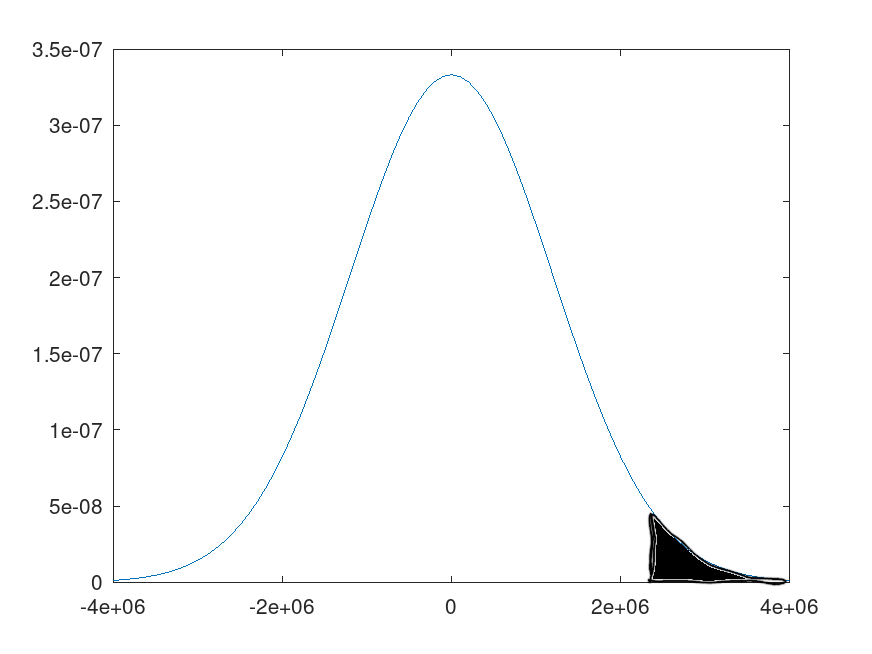
\includegraphics[width=.5\textwidth]{Prob1.png}

        \end{tabular}

        \begin{flushleft}
          \begin{tabular}{|c|}
            \hline
            \textbf{Conclude}\\
            \hline
          \end{tabular}
        \end{flushleft}

        Because .0457 $<$ .05, Lavrentiy Beria may reject the null hypothesis. Thus, it is clear that there were more Soviet losses than allied losses present in the second World War.

\end{enumerate}

\end{document}

